\documentclass[12pt]{exam}
\usepackage[utf8]{inputenc}		% Caracteres latinos
\usepackage[spanish]{babel}		% Idioma español
\usepackage{geometry}			% Organizar el documento
\usepackage{graphicx}			% Incluir gráficos
\usepackage{makecell}			% Para personalizar las celdas de una tabla
\usepackage[nohdr]{mathexam}	% Añadimos el paquete mathexam (sin header)
\usepackage{amsmath}
\usepackage{amsfonts}
\usepackage{amssymb}
\usepackage{mathtools}
\usepackage{tikz,pgfplots}
\usepgfplotslibrary{polar}
\usepackage[shortlabels]{enumitem}
 \renewcommand{\baselinestretch}{1.5}
\usepackage{mathtools}
\usepackage{bm}
\usepackage{esvect}
\usepackage[fleqn]{mathtools}
\usepackage{relsize}
\usepackage{multirow}
\usepackage{multicol}
\usepackage[document]{ragged2e}
 \usepackage{textpos}
\usepackage{tcolorbox}
\usepackage{hyperref}

%\usepackage[]{mathptmx}        % A free version o Times Roman with mathematical symbols
%\usepackage{pzc}               % fuente cursiva (conjuntos) Zapf Chancery
%\usepackage{showframe}
%\usepackage{lipsum}

% DOCUMENTACIÓN DE LA CLASE EXAM
% http://ftp.inf.utfsm.cl/pub/tex-archive/macros/latex/contrib/exam/examdoc.pdf
% DOCUMENTACIÓN DE LA CLASE MATHEXAM
% http://ctan.dcc.uchile.cl/macros/latex/contrib/mathexam/doc/mathexam.pdf

% Definimos la geometría de la primera página
\geometry{
	a4paper,                    % Tamaño del documento
	hmargin = {1.7cm, 1.6cm}, 	% Margen horizontal izquierdo, derecho
	vmargin = {1cm, 1cm},	    % Margen vertical superior, inferior
	headsep = 4mm,				% Separación entre el encabezado y el texto
	head = .2cm,				% Tamaño del encabezado
	% marginparsep = 5mm, 		% Seperación entre las notas y el texto
	% marginpar = 1.5cm,		% Tamaño de las notas
	includeall,                 % incluye el encabezado, footer y notas dentro del tamaño del documento
	nomarginpar,	            % Elimina las notas
	foot = 1cm,                 % Tamaño del footer
	twoside,                	% Habilita el modo de impresión a doble cara
}

\selectlanguage{spanish}        % Selecciona el idioma
\spanishdecimal{.}

%\pagestyle{headandfoot}         % Nuestro examen tendrá encabezado y pié

% DEFINIMOS EL ENCABEZADO
%\header{
%\begin{tabular}{l c c c l}
%            \makecell{\includegraphics[height=2.5cm]{logo.png}} &
%            \makecell{\textbf{IPEA 215} \\Raúl Scalabrini Ortiz} &
%            \makecell{Examen} &
%            \makecell{Curso\\1er Año} &
%             \makecell[l]{Apellido y %Nombre:\enspace\makebox[2in]{\hrulefill}\\Fecha: \today}
%        \end{tabular}}{}{}

% DEFINIMOS EL PIE
%\rfoot{Página \thepage\ de \numpages}
\newcommand{\iuni}{\pmb{\hat{\imath}}}
\newcommand{\juni}{\pmb{\hat{\jmath}}}
\newcommand{\kuni}{\pmb{\hat{k}}}
\renewcommand{\sin}{\,\text{sen}\,}

% DOCUMENTO
\begin{document}

\centering


\Large 
\textbf{\huge Tarea 2\\ \large Técnicas analíticas}

\small
Fecha de entrega lunes 25 de Octubre
\vskip10pt
% \flushleft
% \begin{tcolorbox}
% LEE ANTES DE COMENZAR LA TAREA
% \begin{itemize}
%     \item Se califica sobre 10 por lo que es posible obtener 13 si se realizan también los ejercicios opcionales.
%     \item El ejercicio opcional puede sustituir a uno y solo uno de los ejercicio del bloque previo.
%     \item Subir el archivo en \textbf{PDF} a la plataforma con las páginas numeradas.

% \end{itemize}
% \end{tcolorbox}
\normalsize

\pointpoints{punto}{puntos}
\pointformat{\bfseries\boldmath(\thepoints)}
\vskip10pt

    
    \begin{questions}
     % 1 %
     \question% S2.2 e2,3,4,5,6 pp46 S2.3 e3,4,5,6 pp54 S2.4 e1,3,4,7,8 pp65
     Determina para cada una de las siguientes ecuaciones si son: separables, lineales, exactas o ninguna de las anteriores. Justifica tu respuesta. \textbf{No} resuelvas la ecuación diferencial.
     \begin{enumerate}[a)]
         \item $\frac{dy}{dx}=\sin(x+y)$
         \item $\frac{dy}{dx}=\frac{ye^{x+y}}{x^2+2}$
         \item $\frac{ds}{dt}=t\ln(s^{2t})+8t^2$
         \item $s^2+\frac{ds}{dt}=\frac{s+1}{st}$
         \item $(xy^2+3y^2)dy-2xdx=0$
         \item $x\frac{dx}{dt}+t^2x=\sin t$
         \item $3t=e^t\frac{dy}{dt}+y\ln t$
         \item $(t^2+1)\frac{dy}{dt}=yt-y$
         \item $3r=\frac{dr}{d\theta}-\theta^3$
         \item $(x^2y+x^4\cos x)dx-x^3dy=0$
         \item $(ye^{xy}+2x)dx+(xe^{xy}-2y)dy=0$
         \item $\sqrt{-2y-y^2}dx+(3+2x-x^2)dy=0$
         \item $\theta dr+(3r-\theta-1)d\theta=0$
         \item $[2x+y\cos(xy)]dx+[x\cos(xy)-2y]dy=0$
     \end{enumerate}
    
     % 2 %
     \question% S2.2 e13,15,18,23 pp46
     Resuelve las siguientes ecuaciones y problemas con valor inicial.
     \begin{enumerate}[a)]
     	\item $\frac{dx}{dt}+x^2=x$
        \item $y^{-1}dy+ye^{\cos x}\sin xdx=0$
        \item $\frac{dy}{dx}=(1+y^2)\tan x$, con $y(0)=\sqrt{3}$
        \item $\frac{dy}{dx}=2x\cos^2y$, con $y(0)=\pi/4$
     \end{enumerate}

     % 3 %
     \question% S2.2 e29
     Considera la ecuación $dy/dx=y^{1/3}$ y el hecho de que por el método de ecuaciones separables no siempre podemos obtener todas las soluciones.
     \begin{enumerate}[a)]
     	\item	Usa el método de separación de variables para mostrar que $y=\left(\frac{2x}{3}+C\right)^{3/2}$ es una solución.
        \item	Muestra que el problema con valor inicial $dy/dx=y^{1/3}$ y $y(0)=0$ se satisface cuando $C=0$ y $y=(2x/3)^{3/2}$ para $x\geq0$.
        \item	Muestra que la función constante $y\equiv0$ satisface el problema con el valor inicial del inciso b) y por lo tanto este problema con valor inicial no tiene solución única.
         \item	Muestra que las condiciones del Teorema de Existencia y Unicidad no se satisfacen.
     \end{enumerate}
Obs: La solución $y\equiv0$ se perdió debido a la división entre 0 en el proceso de separación.

     % 4 %
     \question% S2.2 e33 pp48
     Supón que una solución salina con 0.3 kg de sal por litro se introduce en un tanque que contenía originalmente 400 litros de agua y 2 kg de sal. Si la solución entra a razón de 10 litros/minuto, la mezcla se mantiene uniforme revolviéndola, y la mezcla sale con la misma razón, determina la masa de sal en el tanque después de 10 minutos usando separación de variables. (Hint: si $A$ son los kilogramos de sal en el tanque, a $t$ minutos después de iniciar el proceso, aplica el planteamiento: razón de incremento A=razón de entrada - razón de salida)
    
    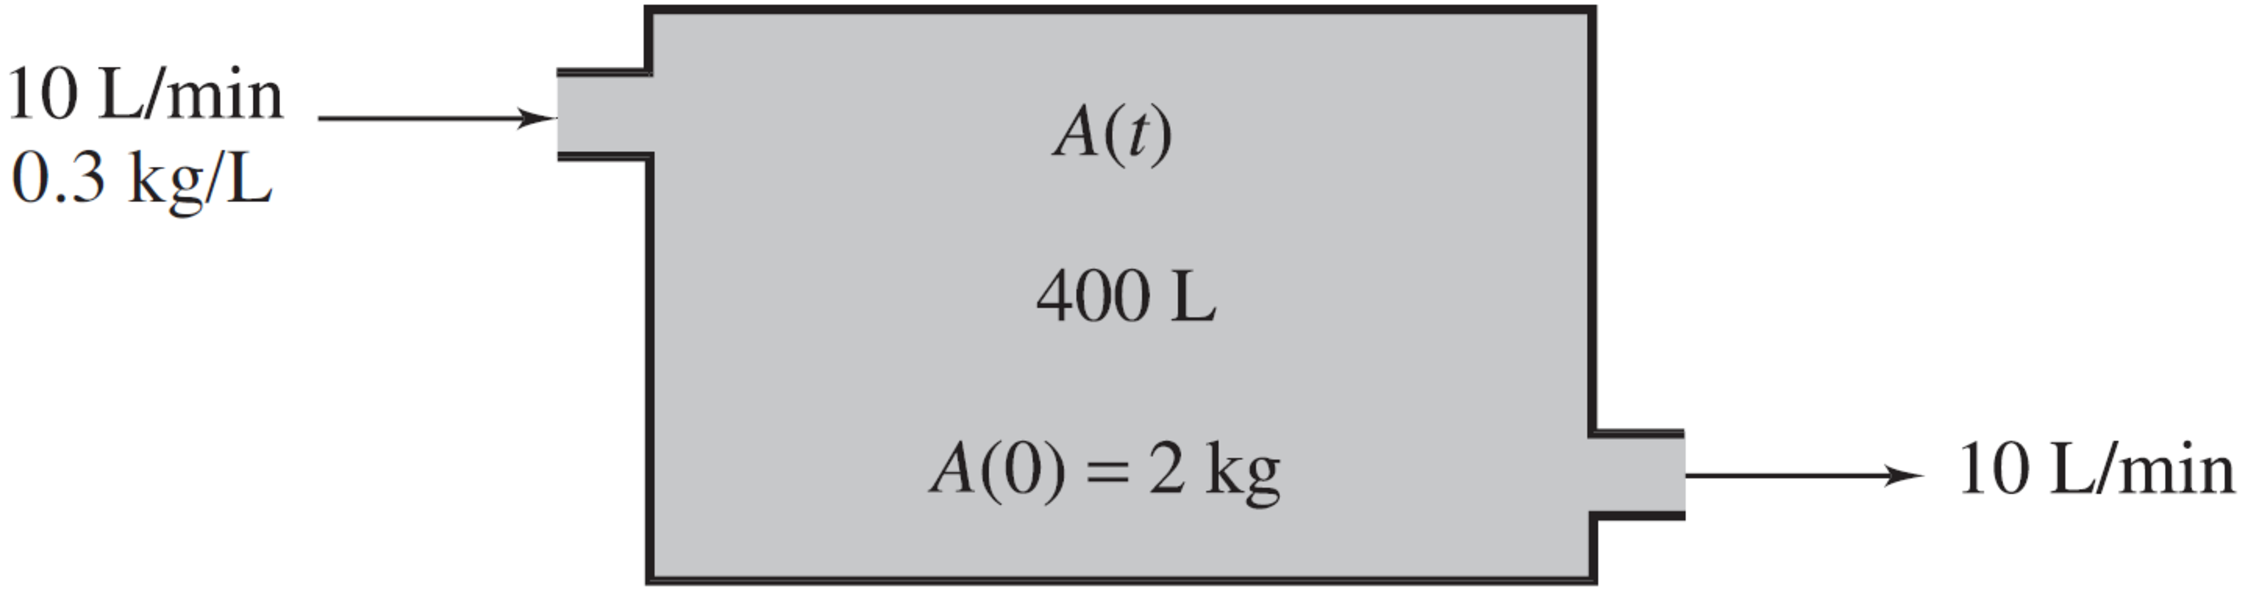
\includegraphics[scale=.4]{F1T2.pdf}


     % 5 %
     \question% S2.2 e34 pp48
     Según la ley de enfriamiento de Newton, al introducir un objeto a temperatura $T$ en un medio con temperatura $M$, la razón de cambio de $T$ es proporcional a la diferencia de temperatura $M-T$ siguiendo la ecuación diferencial $\frac{dT}{dt}=k(M-T)$:
     \begin{enumerate}[a)]
     \item	Resuelve la ecuación diferencial en términos de $T$
     \item	Si un termómetro marca $100°F$ y se coloca en un medio con temperatura constante de $70°F$.  Después de 6 min el termómetro marca $80°F$. ¿Cuál es la lectura después de 20 minutos?
     \end{enumerate}


     % 6 %
     \question%S2.3 e9,16,20,22 pp55
     Obtén la solución general para las ecuaciones sin valor inicial indicado y resuelve los problemas con valor inicial si esta indicado:
     \begin{enumerate}[a)]
     \item	$\frac{dr}{d\theta}+r\tan\theta=\sec\theta$
     \item	$(x^2+1)\frac{dy}{dx}=x^2+2x-1-4xy$
     \item	$\frac{dy}{dx}+\frac{3y}{x}+2=3x$, con $y(1)=1$
     \item	$\sin x\frac{dy}{dx}+y\cos x=x\sin x$, con $y(\pi/2)=2$
     \end{enumerate}

     % 7 %
     \question%S2.3 e23 pp55
     Suponiendo la ecuación de decaimiento $\frac{dy}{dt}=40e^{-20t}-ky$, donde $k=5/s$. Determina la masa $y(t)$ para $t\geq0$ si inicialmente $y(0)=10kg$.

     % 8 %
     \question% S2.3 e35 pp57
     Supón que una solución salina con 0.2 kg de sal por litro se introduce en un tanque que contiene inicialmente 500 litros de agua y 5 kg de sal. La solución entra al tanque a razón de 5 L/min. La mezcla se mantiene uniforme revolviéndola, y sale del tanque a razón de 5 L/min.

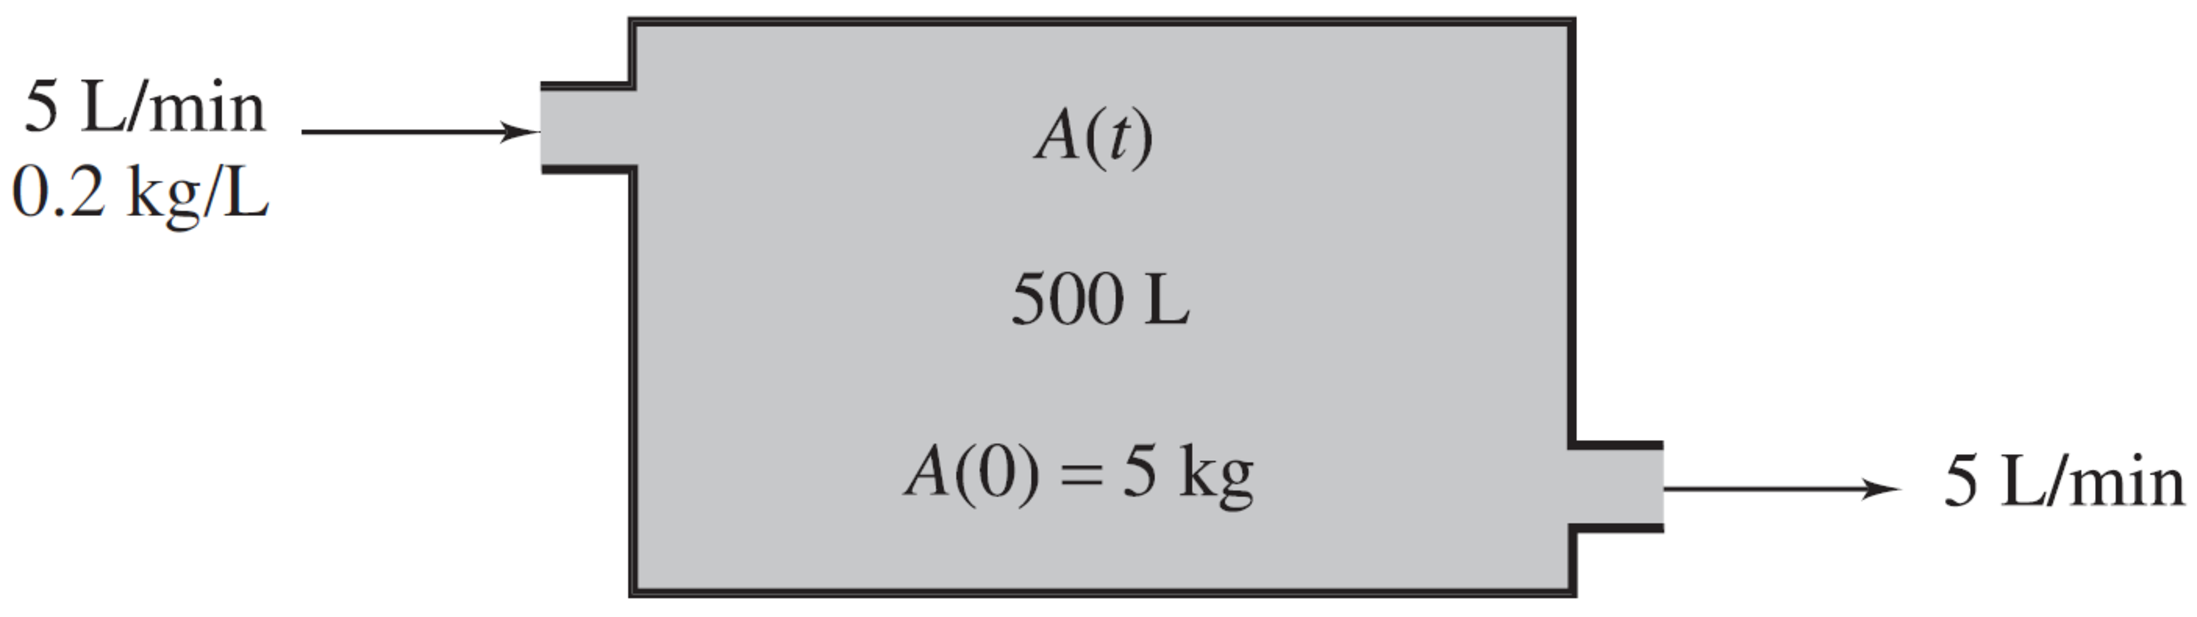
\includegraphics[scale=.34]{F2T2.pdf}

\begin{enumerate}[a)]
	\item	Determina la concentración en kilogramos/litros de sal en el tanque después de 10 minutos viendo al modelo como una ecuación lineal.
    \item Después de 10 minutos aparece en el tanque una fuga a razón de 1 L/min. ¿Cuál será la concentración (en kg/L) de sal en el tanque después de 20 minutos a partir del inicio de la fuga?
    
    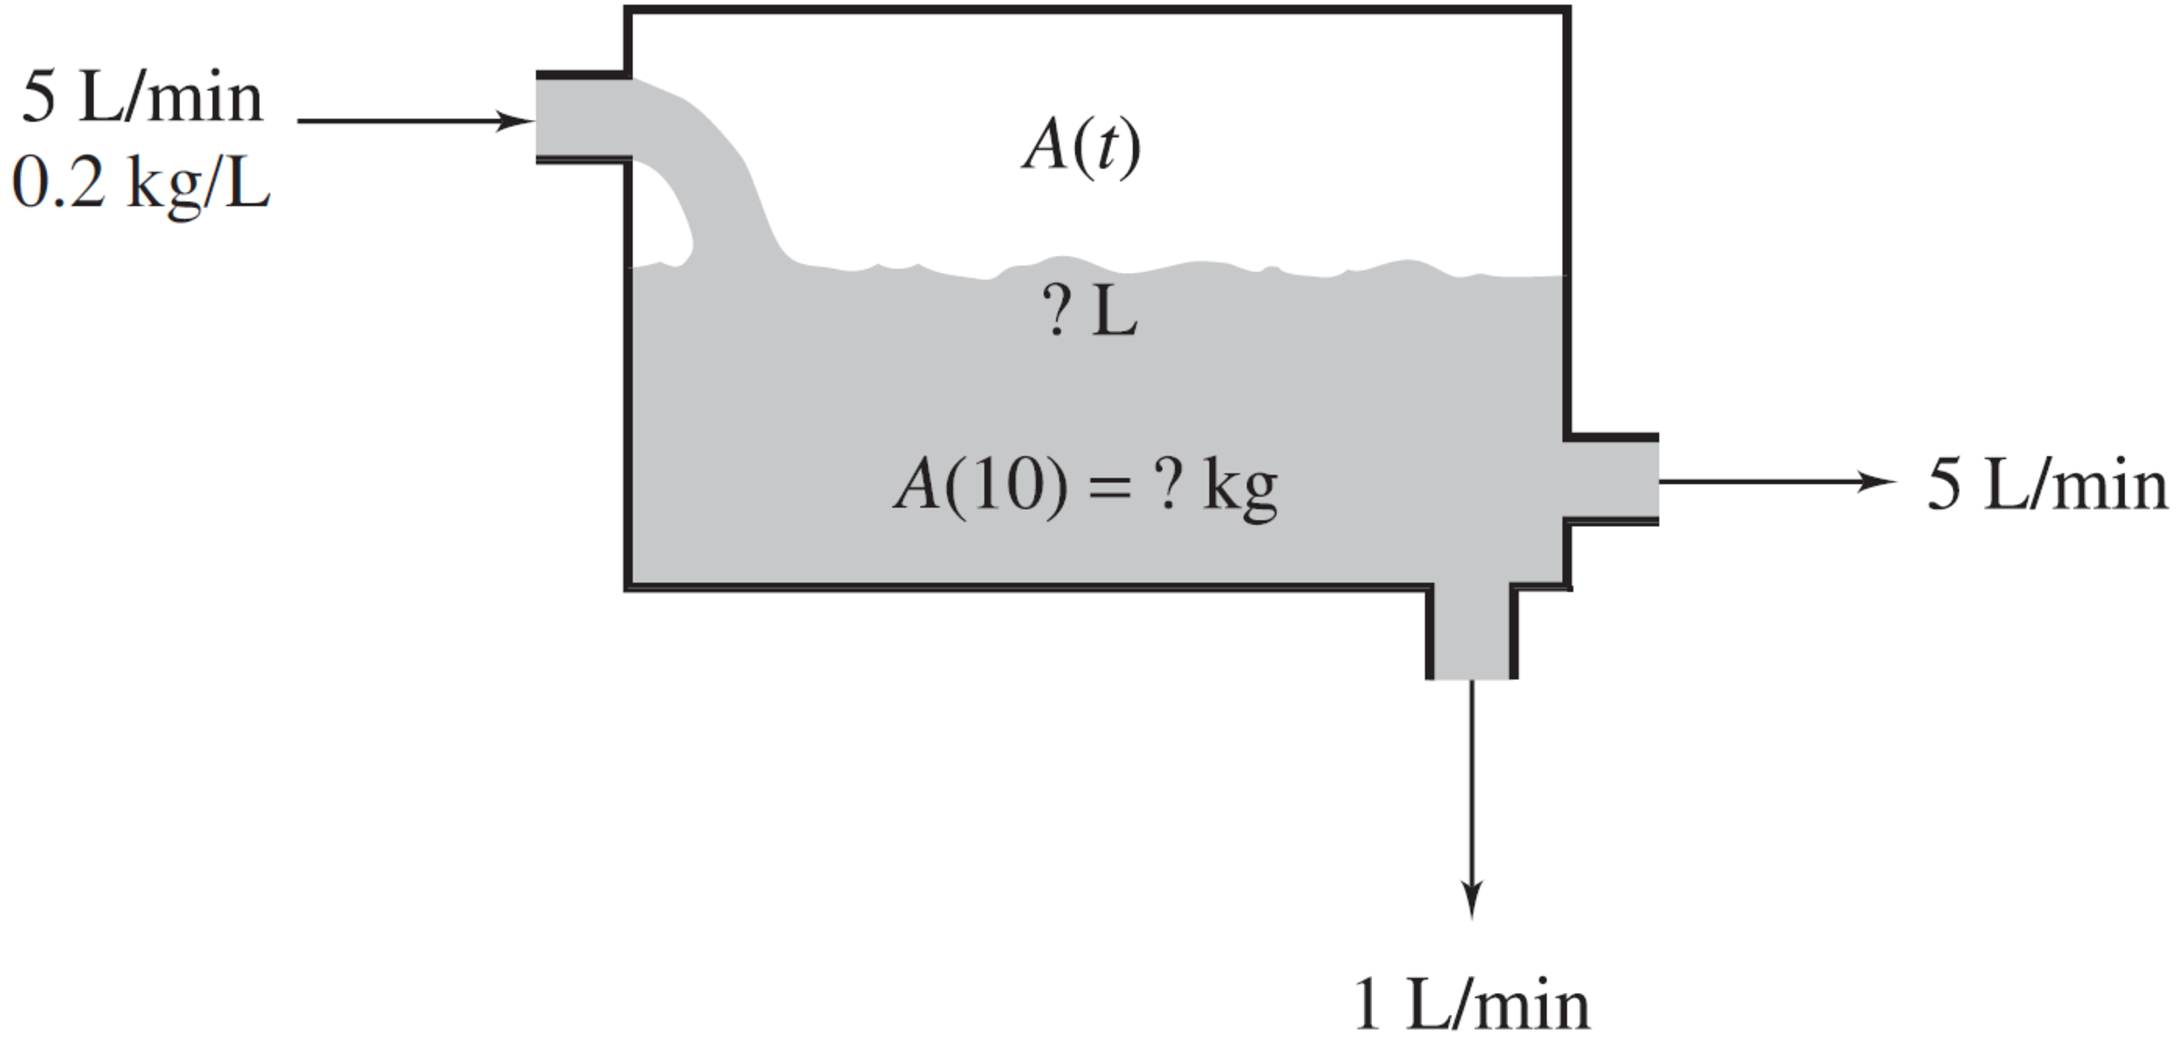
\includegraphics[scale=.34]{F3T2.pdf}
    
\end{enumerate}

     % 9 %
     \question% S2.4 e27 pp66
     \item	$(x^2+1)\frac{dy}{dx}=x^2+2x-1-4xy$
     \begin{enumerate}[a)]
     	\item	$M(x,y)dx+(\sec^2y-x/y)dy=0$
        \item	$M(x,y)dx+(\sin x\cos y-xy-e^{-y})dy=0$
     \end{enumerate}

     % 10 %
     \question% S2.4 e14,15,26 pp66
      Si las siguiente ecuaciones son exacta, resuélvelas.
      \begin{enumerate}[a)]
      	\item	$e^t(y-t)dt+(1+e^t)dy=0$
        \item	$\cos\theta dr-(r\sin\theta-e^{\theta})d\theta=0$
        \item	$(\tan y-2)dx+(x\sec^2y+1/y)dy=0$, con $y(0)=1$
      \end{enumerate}





        \end{questions}
        \vskip30pt
%  \RaggedRight
%  PUNTO EXTRA
 
%  Encuentra el volumen del sólido $S$ como la diferencia entre dos volúmenes. $S$ es el sólido encerrado por los cilindros parabólicos $y=1-x^2$, $y=x^2-1$ y las planos $x+y+z=2$, $2x+2y-z+10=0$.
 
    
%     \newpage



% Geometría para la otra carilla
\newgeometry{
	hmargin = {1.5cm, 1.5cm},
	vmargin = {5cm, 1cm},
	%nofoot,			% Elimina el pié
	nohead,			% Elimina el encabezado
	nomarginpar,	% Elimina las notas
	includeall,
}% \savegeometry{geometria_1}

\pagestyle{foot}    % El estilo de ésta página sólo constará de pié de página
\runningfooter{}{}{Página \thepage\ de \numpages}


%\lipsum[1-5]

% \restoregeometry
% \loadgeometry{geometria_1}


\end{document}
     \item	$(x^2+1)\frac{dy}{dx}=x^2+2x-1-4xy$

\usepackage{tcolorbox}

